\clearpage
\section{Mobile-D}
\subsection{Definicion \cite{B30}}
Mobile-D es una metodología de desarrollo ágil enfocada al desarrollo de aplicaciones móviles. Está basada en otras tres metodologías:
\begin{itemize}
	\item Extreme Programming.
	\item Crystal.
	\item Rational Unified Process.
\end{itemize}
Mobile-D posee las siguientes características:
\begin{itemize}
	\item \textbf{Fases y ritmo}. Los proyectos son desarrollados en iteraciones que comienzan con un día de planeación.
	\item \textbf{Línea de arquitectura}. La construcción de las aplicaciones se hace con patrones de arquitectura y modelado ágil.
	\item \textbf{Desarrollo de pruebas móviles}. Realiza pruebas automatizadas.
	\item \textbf{Integración continua}. Reduce los tiempos de entrega.
	\item \textbf{Programación en pares}. La programación y las pruebas de la aplicación se realizan en parejas.
	\item \textbf{Métricas}. Durante el desarrollo se pueden obtener datos que puedan medir el rendimiento de los procesos de desarrollo.
	\item \textbf{Proceso de software ágil}. Al final de cada iteración se pueden organizar reuniones con el objetivo de mejorar el proceso de desarrollo.
	\item \textbf{Contacto con cliente}. El cliente participa en las etapas de planeación y liberación de las iteraciones.
	\item \textbf{Enfoque al usuario}. Se hace énfasis en la identificación de las necesidades del usuario final.
\end{itemize}

El desarrollo a través de ésta metodología se realiza a través de iteraciones, y cada una de estas contiene cinco etapas (véase Figura 2.8):
\begin{figure}[h!]
	\centering
	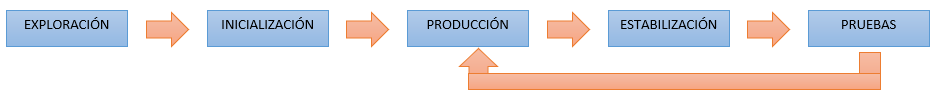
\includegraphics[width=16cm]{imagenes/marcoteorico/mobiled.png}
	\caption{Estructura de Mobile-D. Elaboración propia.}
	\label{fig:mobiled}
\end{figure}
\begin{itemize}
	\item \textbf{Exploración}. El propósito de esta fase es establecer las bases iniciales para el desarrollo del proyecto. Aquí se definen a los involucrados en el proyecto y su participación, el alcance de la aplicación, las iteraciones que se harán en total para todo el proyecto, y pruebas de contexto del software que se planea emplear. Ésta fase se realiza solamente en la primer iteración (iteración 0).
	\item \textbf{Inicialización}. En ésta fase se define el entorno de trabajo del proyecto (las herramientas, versiones y dispositivos que se usarán) y la arquitectura que tendrá el sistema. De igual forma, ésta fase sólo se realiza en la primer iteración (iteración 0).
	\item \textbf{Producción}. En ésta fase se realiza la programación del sistema. Se desarrolla lo planeado en la etapa de exploración.
	\item \textbf{Estabilización}. Si lo desarrollado en la iteración consta de varios módulos, ésta etapa se encarga de unirlos y asegurar la integridad del sistema. Dentro de esta etapa también se realiza la documentación del sistema.
	\item \textbf{Pruebas y correcciones}. Se realizan pruebas a la aplicación verificando que se cumplan los casos de uso, y en caso de haber errores, se corrigen también en esta etapa.
\end{itemize}


